\documentclass[a4paper]{article}
\usepackage[utf8]{inputenc}
\usepackage{amsmath}
\usepackage{graphicx}
\usepackage{caption}
\usepackage{pdfpages}
\setcounter{tocdepth}{4}
\setcounter{secnumdepth}{4}
\setlength\parindent{0pt}
\usepackage{siunitx}
\usepackage{float}
\begin{document}
\usepackage{graphicx}
\title{Weather Report\\\textit{Insights drawn from weather measurements in Sweden} \\ FYTN03}
\author{Leo Zethraeus, 
Piotr Yartsev, Xi-Zhen Liu} % Author name
\date{November 2019} % Date for the report
\maketitle
\newpage
\tableofcontents

\newpage

\section{Introduction}
The Swedish Meteorological and Hydrological Institute (SMHI) routinely records the temperature at various locations in Sweden. In some places, this has been going on for hundreds of years. The goal of this project is to find at least three interesting results from the SMHI data. The Data set consists of sssentially these parameters: Time (in format year-month-day-hour:minute), Temperature, longitude, latitude, altitude. We are using C++ and bash script to clean and process the data, then use ROOT to visualize those data and do further analysis. 

The three main questions we are interested in from these measurements are:
\begin{enumerate}
\item How the annual average temperature in Uppsala changed since the industrial revolution in Sweden, approx 1880?
\item How many days a year is the average temperature in Lulea below 0?
\item Which is the hottest and coldest day most likely to occur in one of the locations in the data set?
\end{enumerate}
The report is set up as follows: Chapter 2 is the introduction of some theories we applied to our questions. Chapter 3 we will talk about how the code works, from reading files to generating plots. Chapter 4 would be the answer of our questions, with some plots. In chapter 5 we discuss our result and explain what we have done.


\section{Theory}



\section{Program/algorithm}

For the program that measures the number of days with a average temperature below 0 each year in Lulea bash was predominately used as it is very good at manipulating strings,  which we thought was very good for this task as after we converted the cvs to a txt file all the files we would deal with in this task would have been txt files with strings.

To extract the data from the cvs we iterated over each line in the file and extracted all lines containing ;G as the G denotes lines that have good data. We remove any characters following the G as it includes text describing the cvs file which we do not need.  




\section{Results}
\begin{enumerate}
\item Q1
\item Q2
\item The warmest and coldest day of each year
\begin{figure}[htp]
    \centering
    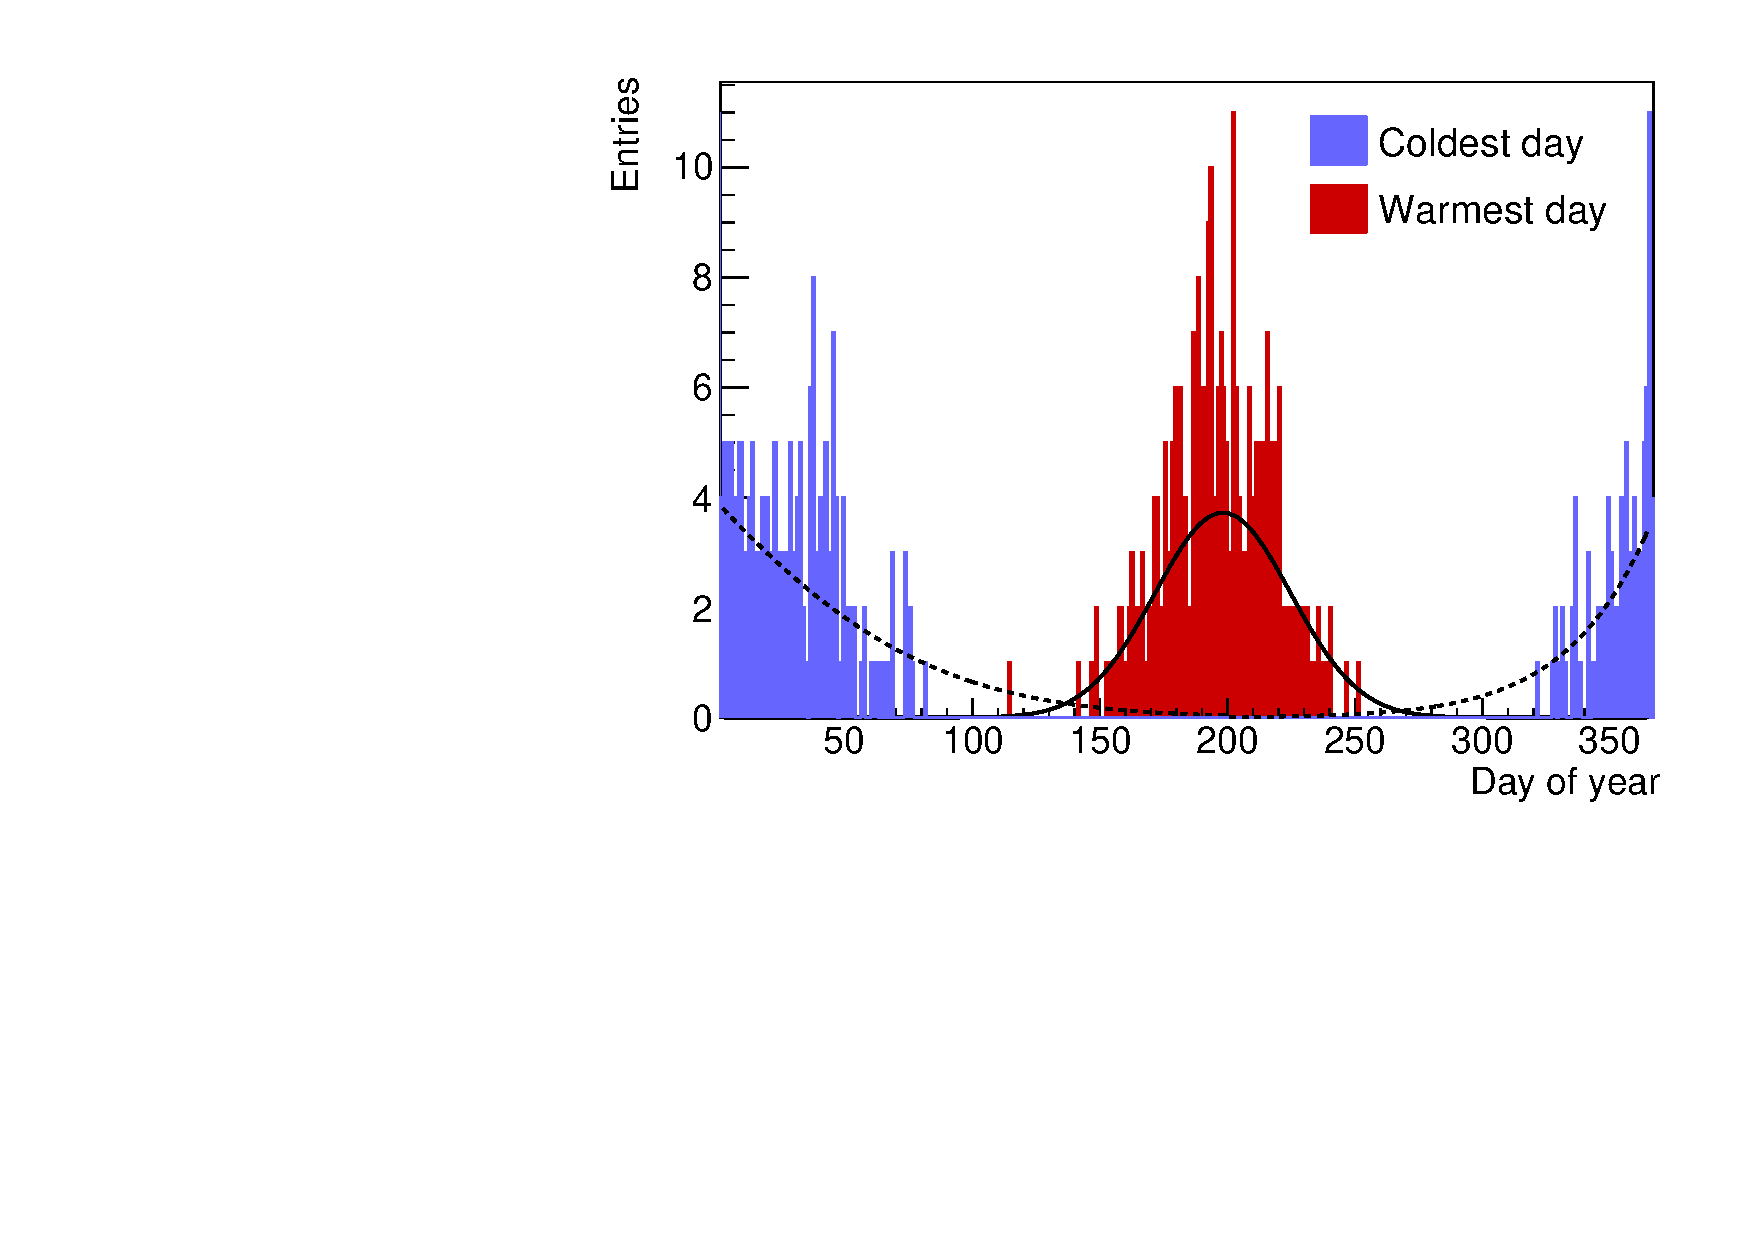
\includegraphics[width=8cm]{./images/hotCold_Upp_final}
    \caption{final histogram}
    \label{fig:hist}
\end{figure}
As the histogram shows, the most likely coldest day is on the end of the year (31/12), and the most likely hottest day is on 13/7.

\end{enumerate}

\section{Discussion}
\begin{enumerate}

\item Q1
\item Q2
\item The warmest and coldest day of each year

The question is to try to find out the possibilites of dates to become the hottest and coldest date. We read the data of Uppsala and then plot the histogram of the occurence for each date being hottest or coldest. 

\begin{figure}[htp]
    \centering
    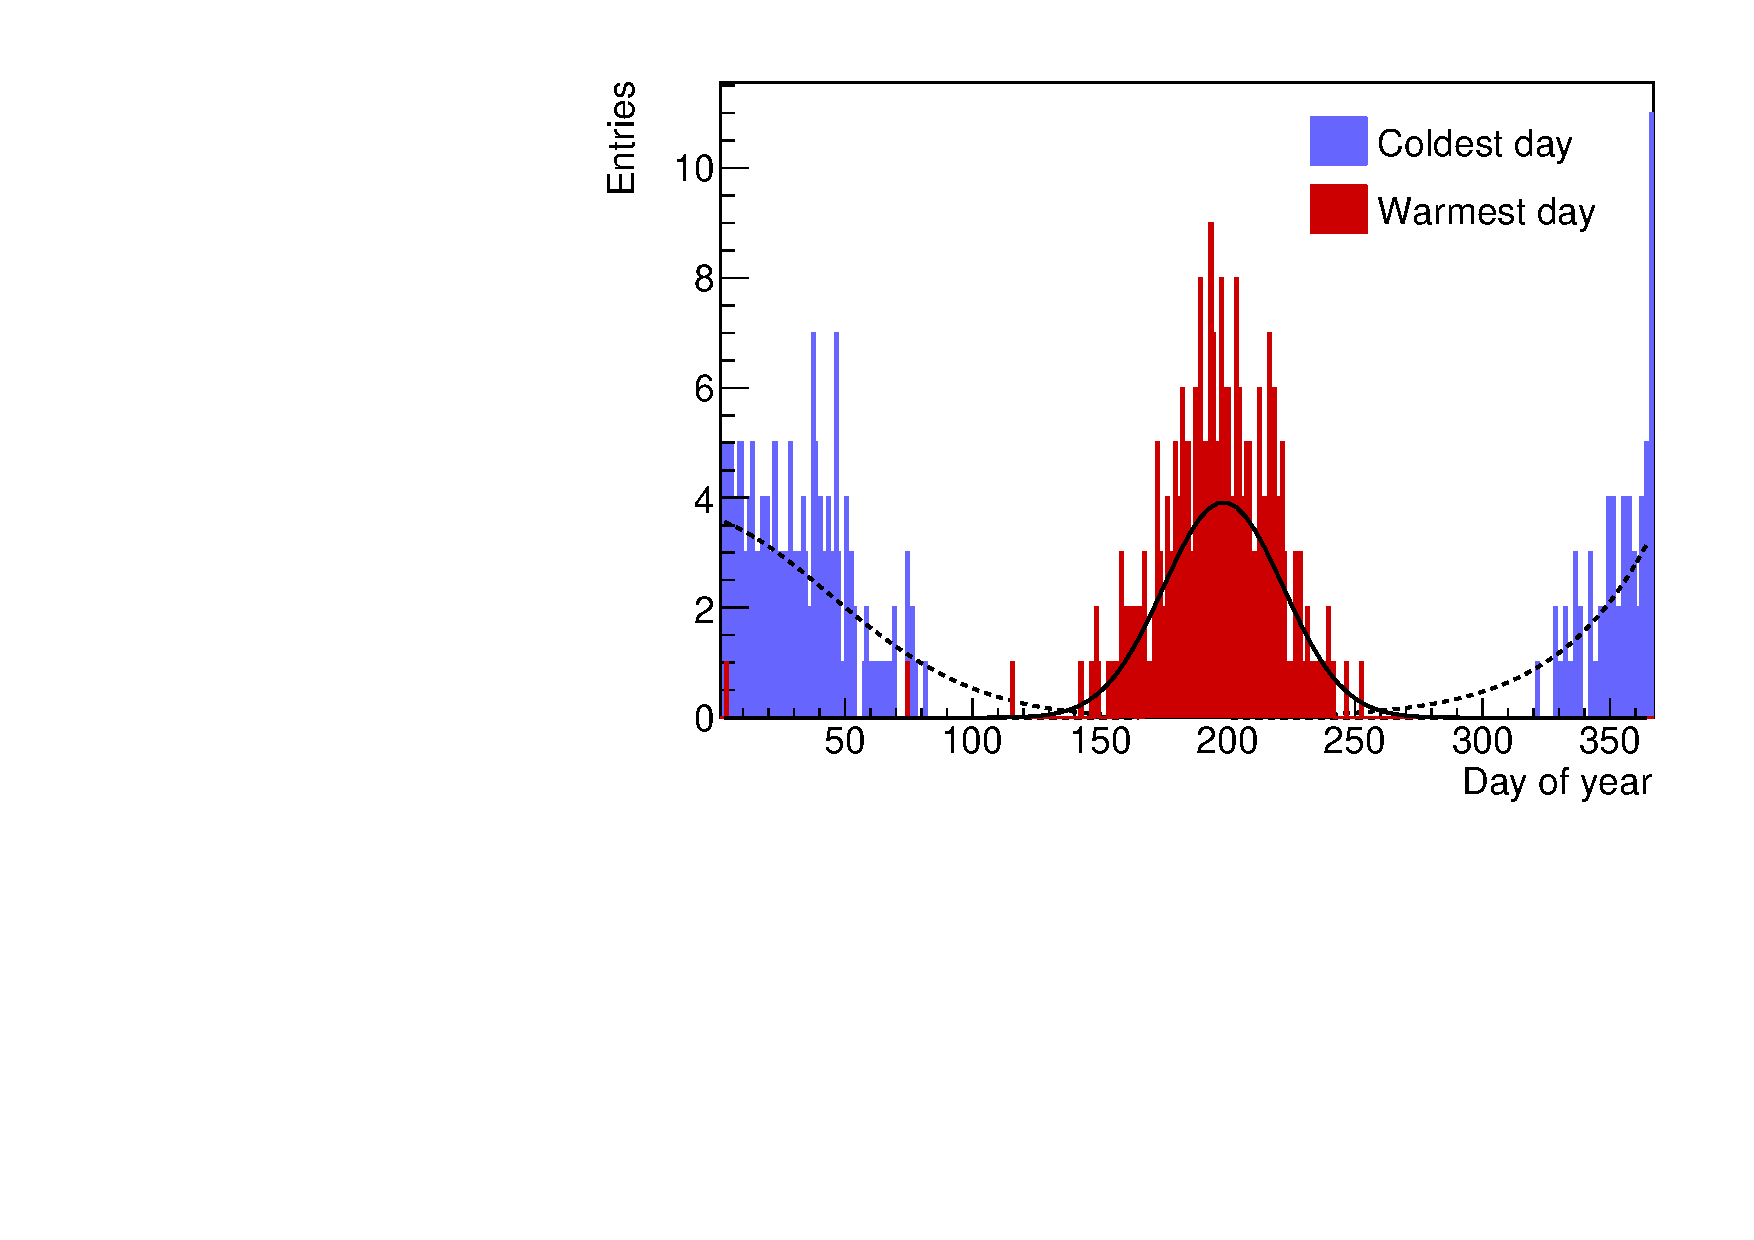
\includegraphics[width=8cm]{./images/hotCold_Upp_prev}
    \caption{first histogram}
    \label{fig:hist}
\end{figure}

We noticed some problem:
\begin{enumerate}
\item There are some coldest date in summer, and also some hottest date in winter, which isn't make sense.
\item Winter is distributed at the first and the end of the year, so we use two Gaussian function to fit on those two parts. However, the plot should be circular in practice. We should take both parts into consideration when we draw fit line.
\end{enumerate}
Then we figured out the cause of the first problem. Because the Uppsala dataset is a combination of some places around Uppsala. For this question, we ignored those places other than Uppsala. This makes the data became uncomplete. For example, data of 1766 are all from Stockholm after April 5, thus the hottest date in 1766 would be April 4, which does not make sense. To solve this, we only accep coldest days which is less than 100 or more than 300 in day of the year, and hottest days which is between 100 and 300 in day of the year.




The graph from the problem where we calculated the nummber of days that had average temperature bellow 0 clearly shows some anomaly in the first few point. It has to do with bad data. The cvs file denoted the quality of the with G for good and bad with Y 



To solve the second problem, we extend the length of the x-axis of histogram to 732, twice of a year. Then we just copy the tail to the front, and also the front to the tail. We plot two Gaussian fit lines for coldest date, one at the front and the other one at the end, and these line must be the same. By doing so, we can take all the coldest date into consideration. Finally, we just need to combine all the fit lines in same plot, and only take from day 1 to day 366 and ignore others.
\begin{figure}[htp]
    \centering
    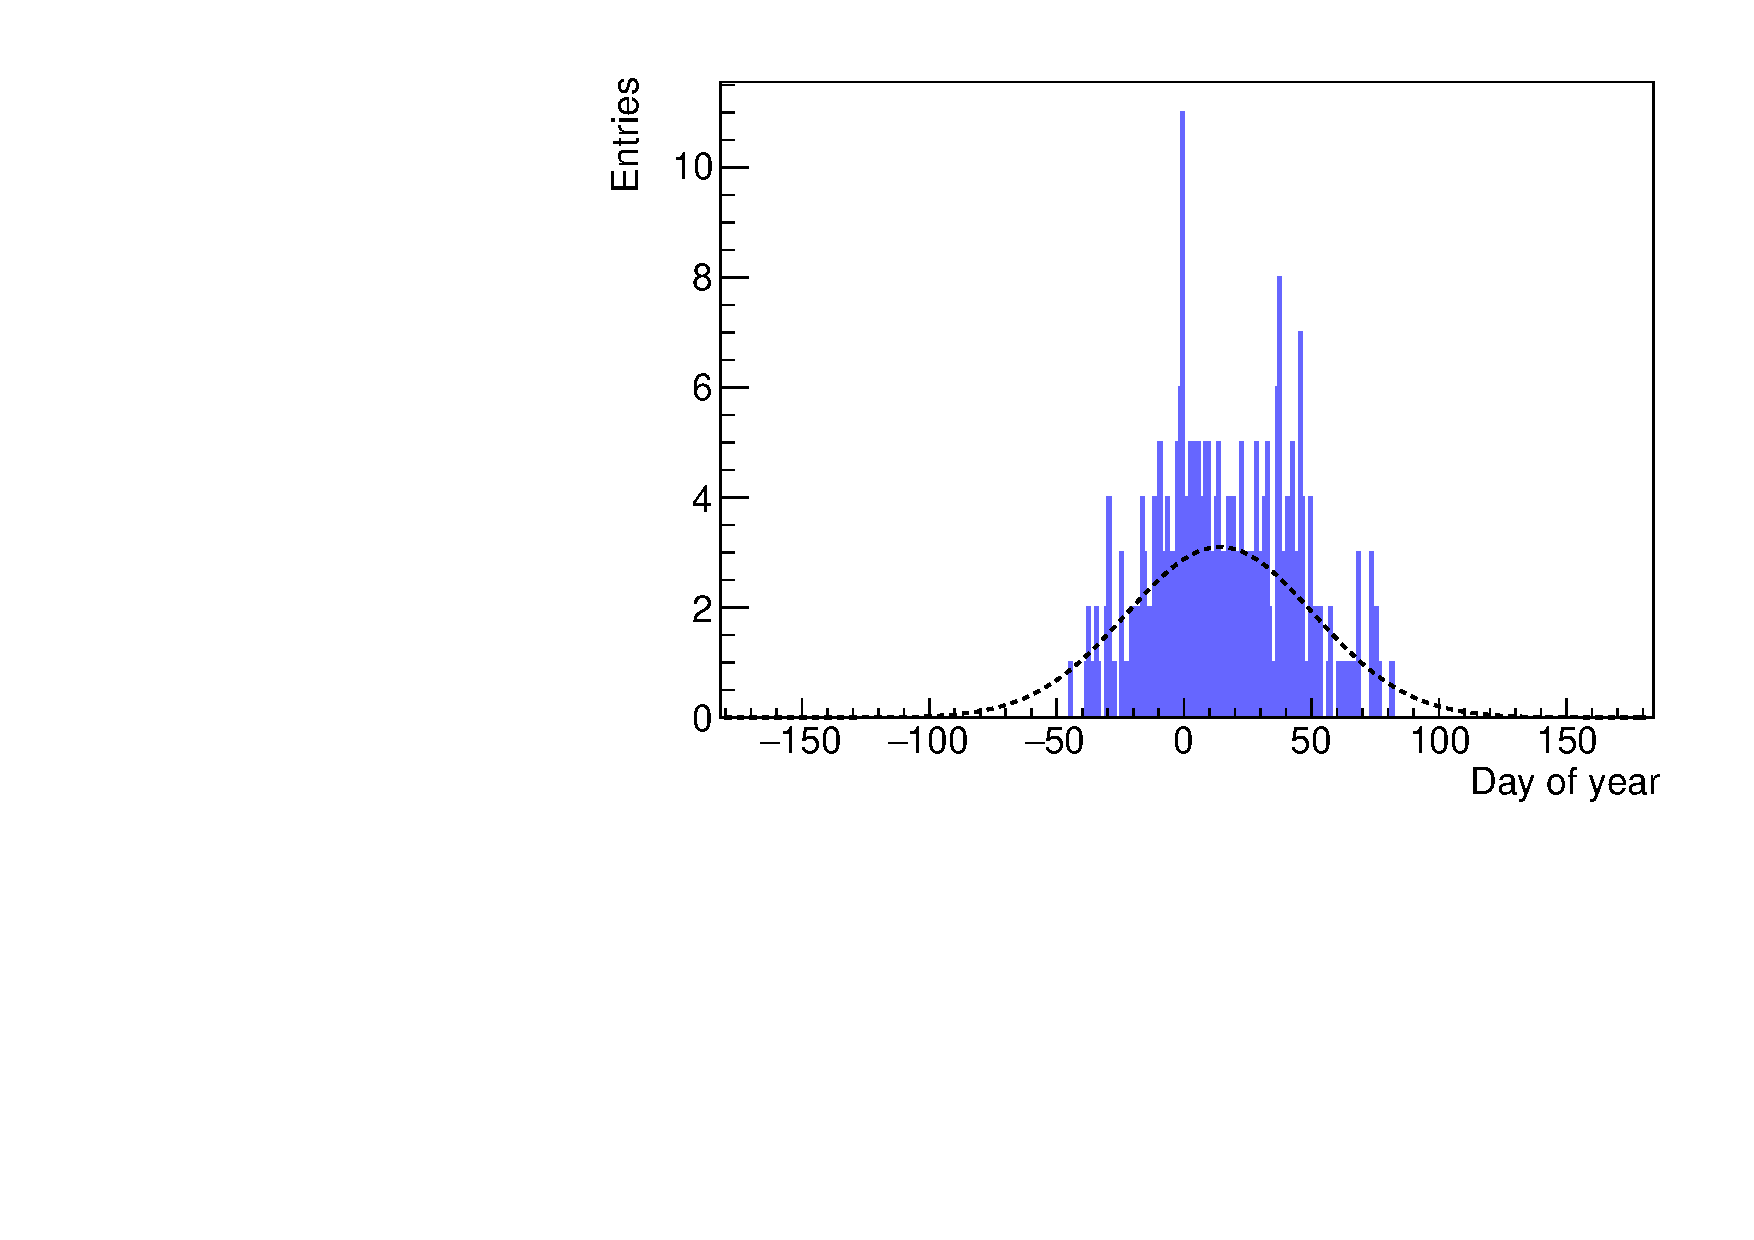
\includegraphics[width=8cm]{./images/hotCold_Upp_cold_1}
    \caption{extended histogram at the begin of the year}
    \label{fig:hist}
\end{figure}
\begin{figure}[htp]
    \centering
    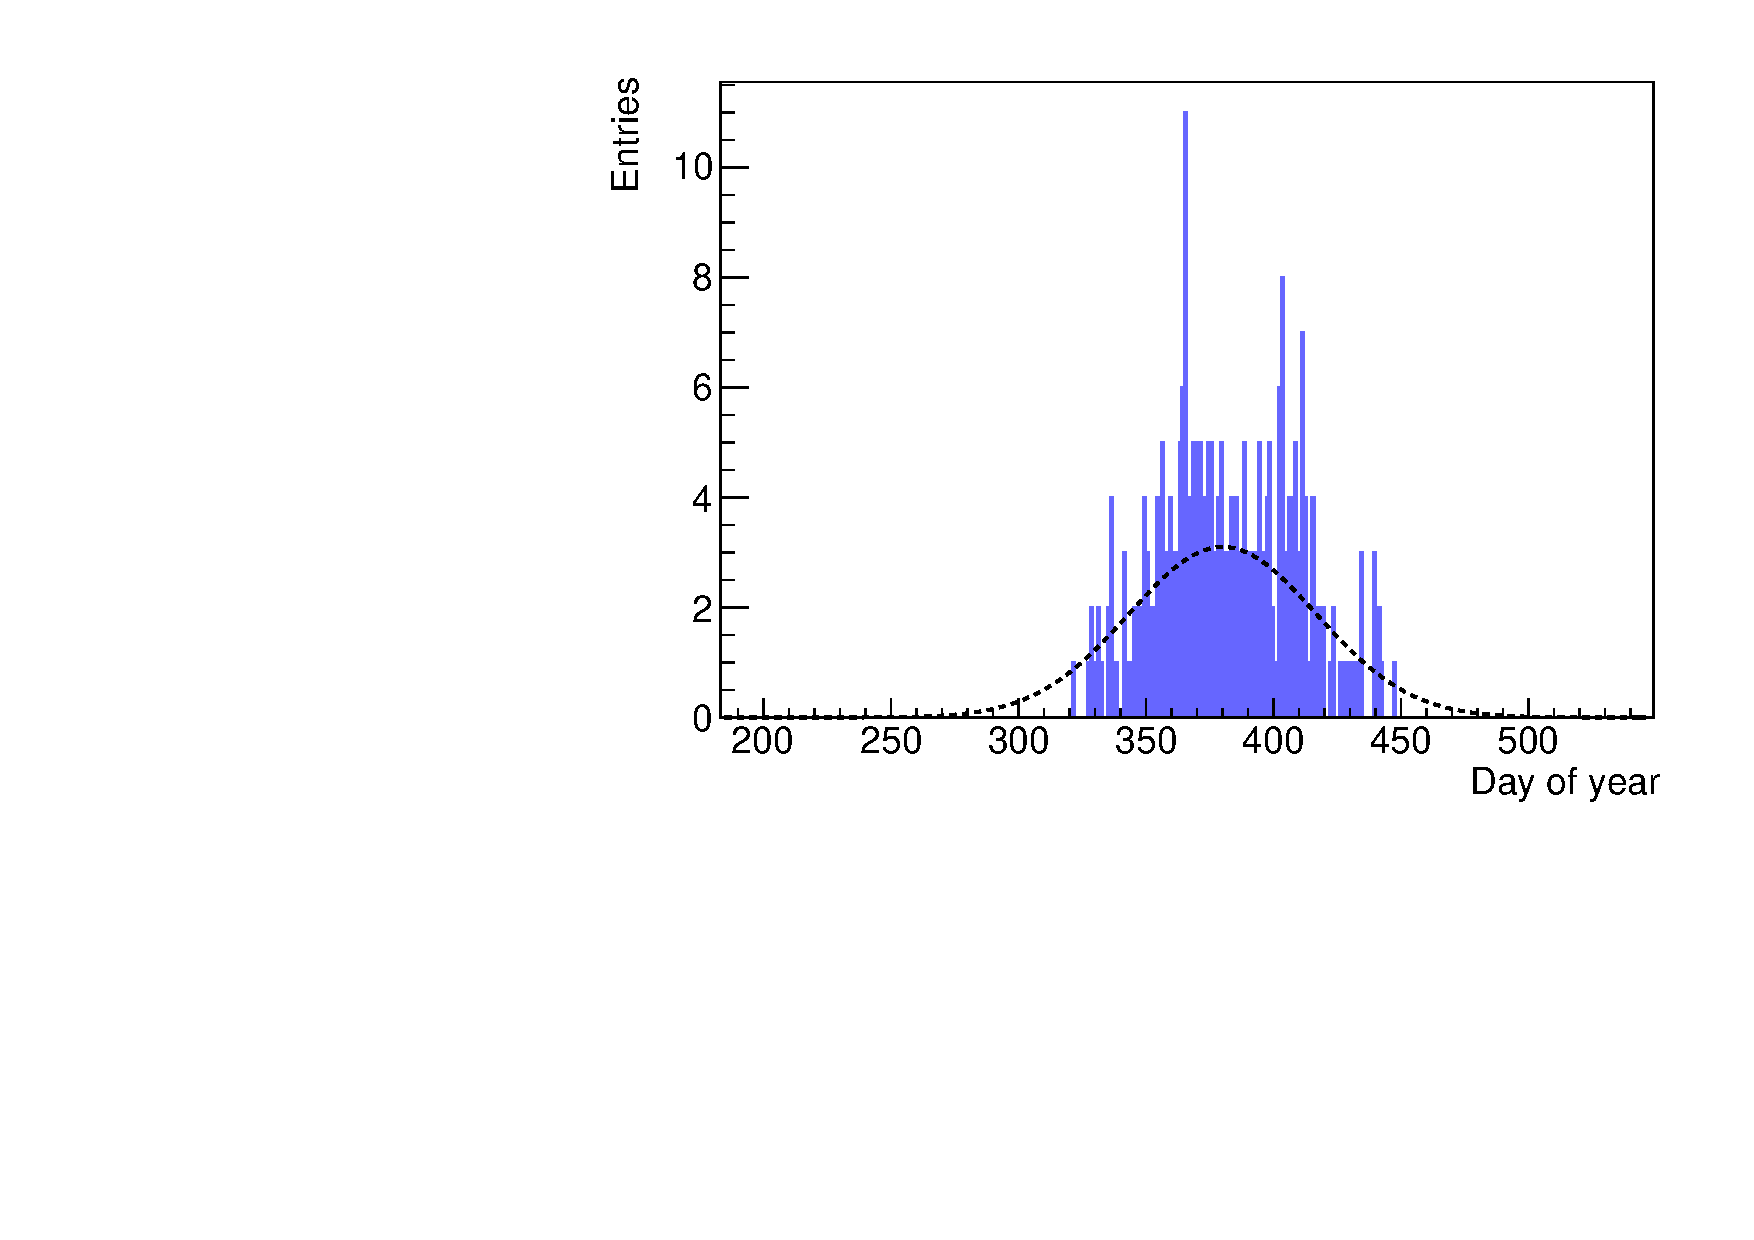
\includegraphics[width=8cm]{./images/hotCold_Upp_cold_2}
    \caption{extended histogram at the end of the year}
    \label{fig:hist}
\end{figure}

The final histogram:
\begin{figure}[htp]
    \centering
    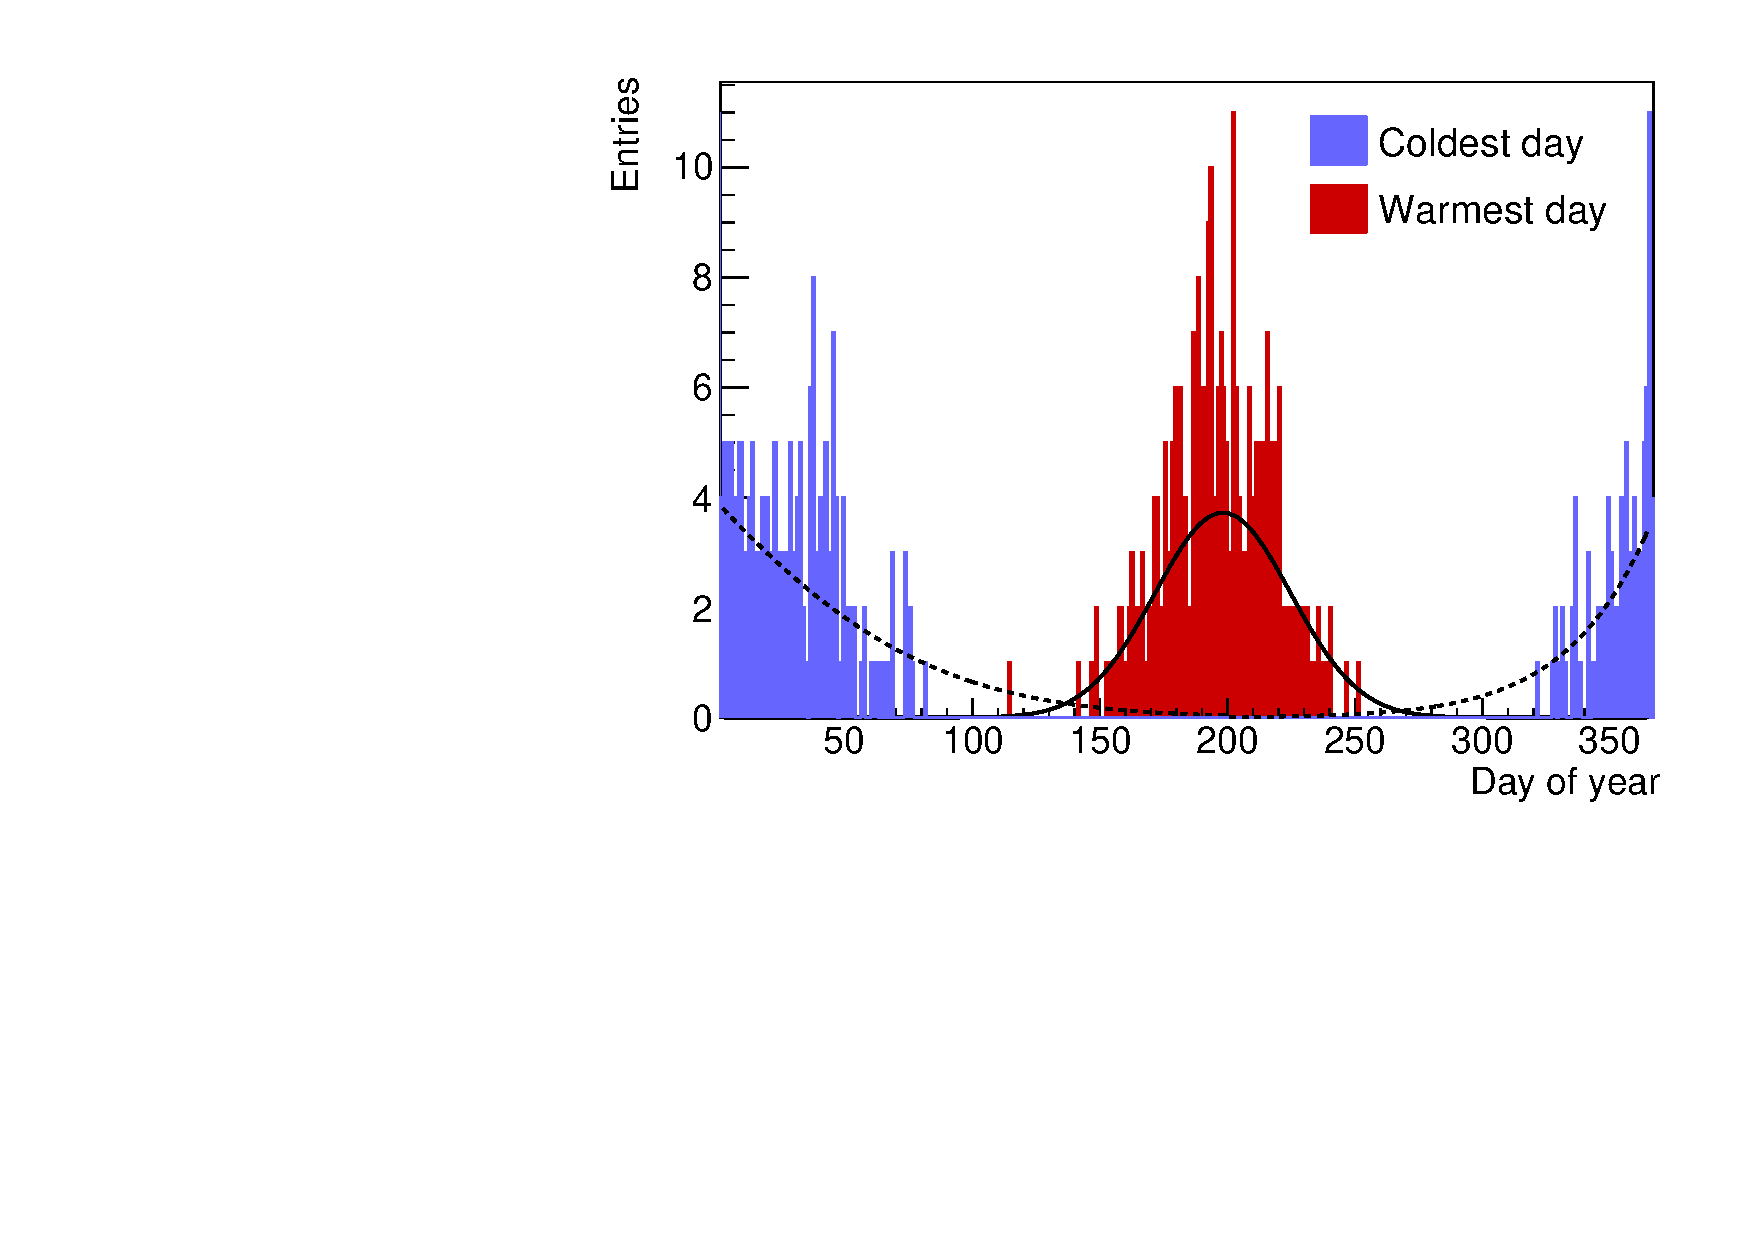
\includegraphics[width=8cm]{./images/hotCold_Upp_final}
    \caption{final histogram}
    \label{fig:hist}
\end{figure}
\end{enumerate}




\end{document}
